% 'Notas de aula não oficiais de MS650 e F620' (c) 2012, 2013 de Raniere Silva
% <ra092767@ime.unicamp.br>
%
% Este trabalho é baseado nos manuscritos das notas de aula do Professor Doutor
% Jayme Vaz Júnior. para as disciplinas MS650, Métodos de Matemática Aplicada
% II, e F620, Métodos Matemáticos da Física II, disponibilizadas em
% http://www.ime.unicamp.br/~vaz/metodos2S12.htm. É permitido a este fazer uso
% deste trabalho para qualquer fim e sem nenhuma restrição.
%
% É permitido fazer uso das criações do espírito presentes neste trabalho
% diretamente relacionadas com os manuscritos das notas de aula do Professor
% Doutor Jayme Vaz Júnior única e exclusivamente para fins educacionais.
%
% Salvo indicação em contrário, este trabalho foi licenciado com a Creative
% Commons Atribuição-CompartilhaIgual 3.0 Não Adaptada. Para ver uma cópia desta
% licença, visite http://creativecommons.org/licenses/by-sa/3.0/.
%
% Este trabalho encontra-se disponível em
% https://github.com/r-gaia-cs/solucoes_ms650_f620.
%
% Este trabalho é distribuído na esperança que possa ser útil, mas SEM NENHUMA
% GARANTIA; sem uma garantia implícita de ADEQUAÇÃO a qualquer MERCADO ou
% APLICAÇÃO EM PARTICULAR.

% Este arquivo inclui o conteúdo de:
%
% * M2S12-13.pdf
% * M2S12-14.pdf

\chapter{Transformadas de Laplace}
\section{Definições e exemplos}
Vamos considerar uma série de potências
\begin{dmath*}
  f(x) = \sum_{k = 0}^{\infty} a_k x^k \condition{$|x| \leq h$.}
\end{dmath*}
Uma forma de generalizar essa série é considerando uma sequência ${\lambda_k}_{k
= 0}^{\infty}$ tal que
\begin{dgroup*}
  \begin{dmath*}
    0 \hiderel{\leq} \lambda_0 \hiderel{<} \lambda_1 \hiderel{<} \lambda_2
    \hiderel{<} \ldots,
  \end{dmath*}
  \begin{dmath*}
    \lim_{k \to \infty} \lambda_k = +\infty
  \end{dmath*}
\end{dgroup*}
e definindo
\begin{dmath*}
  f(x) = \sum_{k = 0}^{\infty} a_k x^{\lambda_k}.
\end{dmath*}

Ocorre, porém, que essa definição requer um cuidado para lidar com os valores
negativos de $x$ pois podemos ter que extrair raízes de $x$ para certos valores
de $\lambda_k$. Para contornar essa situação, vamos considerar $x \geq 0$. Para
garantir isso, vamos tomar $x = \exp(-s)$ e definir
\begin{dmath*}
  F(s) \hiderel{=} f(\exp(-s)) = \sum_{k = 0}^{\infty} a_k \exp(-s \lambda_k).
\end{dmath*}

Essa série é chamada série de Dirichlet. Uma vez que $\Delta k = (k + 1) - k =
1$, temos
\begin{dmath*}
  F(s) = \sum_{k = 0}^{\infty} a_k \exp(-s \lambda_k) \Delta k
\end{dmath*}
e asumindo que $k$ tome valores contínuos e depois o limite $\Delta k \to 0$
segue que
\begin{dmath*}
  F(x) = \int_0^{\infty} a(k) \exp(-s \lambda(k)) \vi{k}.
\end{dmath*}
A transformada de Laplace corresponde ao caso $\lambda(k) = k$.

\begin{defi}
  Dada a função $f(t)$, $0 \leq t \leq \infty$, definimos sua transformadas de
  Laplace como sendo a função $F(s)$ dada por
  \begin{dmath*}
    F(s) \hiderel{=} \mathcal{L}[f(t)] = \int_0^{\infty} f(t) \exp(-s t) \vi{t}
  \end{dmath*}
  definida para os valores de $s$ tais que a integral acima exista. Em geral $s
  \in \mathbb{C}$.
\end{defi}

\begin{exem}
  Vamos calcular a transformada de Laplace para $f(t) = 1$.
  \begin{dmath*}
    \mathcal{L}[1] = \int_0^{\infty} \exp(-s t) \vi{t}
    = \left. - \exp(-s t) / s \right|_0^{\infty}
    = 1 / s \condition{$s > 0$.}
  \end{dmath*}
\end{exem}

\begin{exem}
  Vamos calcular a transformada de Laplace para $f(t) = t^{\alpha}$.
  \begin{dmath*}
    \mathcal{L}[t^{\alpha}] = \int_0^{\infty} t^{\alpha} \exp(-s t) \vi{t}
    = \frac{1}{s^{\alpha + 1}} \int_0^{\infty} y^{\alpha} \exp(-y) \vi{y}
    = \frac{1}{s^{\alpha + 1}} \Gamma(\alpha + 1)
    = \frac{n!}{s^{\alpha + 1}} \condition{$s > 0$.}
  \end{dmath*}
\end{exem}

\begin{exem}
  Vamos calcular a transformada de Laplace para $f(t) = \sin(kt)$.

  Uma vez que
  \begin{dmath*}
    \int \sin(k t) \exp(-s t) \vi{t} = \frac{-1}{k^2 + s^2} \left[ s \exp(-s t)
    \sin(k t) + k \exp(-s t) \cos(k t) \right],
  \end{dmath*}
  temos
  \begin{dmath*}
    \mathcal{L}[\sin(k t)] = \left. \frac{-1}{k^2 + s^2} \left[ s \exp(-s t) + k
    \exp(-s t) \cos(k t) \right] \right|_0^{\infty}
    = \frac{-1}{k^2 + s^2} [-k]
    = \frac{k}{k^2 + s^2} \condition{$s > 0$.}
  \end{dmath*}
  Analogamente,
  \begin{dmath*}
    \mathcal{L}[\cos(k t)] = \frac{s}{k^2 + s^2} \condition{$s > 0$.}
  \end{dmath*}
\end{exem}

\begin{exem}
  Vamos calcular a transformada de Laplace para $f(x) = \exp(a t)$.
  \begin{dmath*}
    \mathcal{L}[\exp(a t)] = \int_0^{\infty} \exp(-s t) \exp(a t) \vi{t}
    = \int_0^{\infty} \exp(- (s - a) t) \vi{t}
    = \left. \frac{\exp(- (s - a) t)}{- (s - a)} \right|_0^{\infty}
    = 1 / (s - a) \condition{$s - a > 0$.}
  \end{dmath*}
\end{exem}

\begin{defi}
  Uma função $f(t)$ definida no intervamo $a \leq t < \infty$ é de ordem
  exponencial $\sigma_0$ ($\sigma_0 \in \mathbb{R}$) se
  \begin{dmath*}
    | \exp(-\sigma_0 t) f(t) | \leq M,
  \end{dmath*}
  onde $M$ é uma constante positiva.
\end{defi}

\begin{teo}
  Se $f(t)$ pe contínua por partes para $0 \leq t < \infty$ e é exponencial de
  ordem $\sigma_0$, então a integral de Laplace
  \begin{dmath*}
    F(s) \hiderel{=} \mathcal{L}[f(t)] = \int_0^{\infty} \exp(-s t) f(t) \vi{t}
  \end{dmath*}
  converge para $\Re(s) > \sigma_0$. Além disso, a integral é absoluta e
  uniformemente convergente para $\Re(s) \geq \sigma_1$ se $\sigma_1 >
  \sigma_0$.
\end{teo}
\begin{proof}
  Para $s = \sigma + i w$, temos que
  \begin{dmath*}
    F_R(s) = \int_0^R \exp(-s t) f(t) \vi{t}.
  \end{dmath*}
  % TODO Terminar a demonstração. M2S12-13.pdf página 5.
\end{proof}

\section{Propriedades}
Antes de começarmos a listar algumas propriedades das transformada de Laplace,
devemos notar que duas funções $f_1(t)$ e $f_2(t)$ tais que
\begin{dgroup*}
  \begin{dmath*}
    f_1(t) = f_2(t) \condition{$0 \leq t < \infty$}
  \end{dmath*}
  \begin{dmath*}
    f_1(t) \neq f_2(t) \condition{$t < 0$}
  \end{dmath*}
\end{dgroup*}
tem a mesma transformada de Laplace. Para evitar essa ambiguidade, vamos
estabelecer que sempre que falamos em uma função $f(t)$ estamos nos referindo à
função $f_N(t)$,
\begin{dmath*}
  f_H(t) \hiderel{=} f(t) H(t) = \begin{cases}
    f(t), & t \geq 0, \\
    0, & t < 0,
  \end{cases}
\end{dmath*}
onde $H(t)$ é a função escada de Heaviside.

\begin{lem}[Translação]
  Se $\mathcal{L}[f(t)] = F(s)$, então para $a < 0$:
  \begin{dgroup*}
    \begin{dmath*}
      \mathcal{L}[f_H(t - a)] = \exp(-a s) F(s),
    \end{dmath*}
    \begin{dmath*}
      \mathcal{L}[\exp(- a t) f(t)] = F(s + a).
    \end{dmath*}
  \end{dgroup*}
\end{lem}
\begin{proof}
  Temos que
  \begin{dmath*}
    \mathcal{L}[f_H(t - a)] = \int_0^{\infty} \exp(-s t) f_H(t - a) \vi{t}
    = \int_0^{\infty} \exp(-s t) f(t - a) H(t - a) \vi{t}
    = \int_a^{\infty} \exp(-s t) f(t - a) \vi{t}
    = \int_0^{\infty} \exp(-s (u + a)t) f(u) \vi{u}
    = \exp(-a s) \mathcal{L}[f(t)].
  \end{dmath*}

  Podemos notar que essa propriedade não vale para $a < 0$ pois nesse caso
  teríamos, se $a < 0$
  \begin{dmath*}
    \int_0^{\infty} \exp(-s t) f_H(t - a) \vi{t} = \int_0^{\infty} \exp(-s t)
    f(t - a) \vi{t}
  \end{dmath*}
  que não guarda a relação acima com $\mathcal{L}[f(t)]$.

  Quanto á outra relação:
  \begin{dmath*}
    \mathcal{L}[\exp(-a t) f(t)] = \int_0^{\infty} \exp(-s t) \exp(-a t) f(t)
    \vi{t}
    = \int_0^{\infty} \exp(-(s + a) t) f(t) \vi{t}
  \end{dmath*}
  e se $\mathcal{L}[f(t)] = F(s)$ existe para $s > \sigma_0$, então para existir
  $\mathcal{L}[\exp(-a t) f(t)]$ devemos ter $s + a > \sigma_0$, ou seja, $a >
  0$.
\end{proof}

\begin{lem}[Derivação]
  As seguintes relações são válidas:
  \begin{dgroup*}
    \begin{dmath*}
      \mathcal{L}[f'(t)] = s \mathcal{L}[f(t)] - f(0),
    \end{dmath*}
    \begin{dmath*}
      F'(s) = - \mathcal{L}[t f(t)].
    \end{dmath*}
  \end{dgroup*}
\end{lem}
\begin{proof}
  Temos que
  \begin{dmath*}
    \int_0^{\infty} \exp(-s t) f'(t) \vi{t} = \left. \exp(-s t) f(t)
    \right|_0^{\infty} + s \int_0^{\infty} \exp(-s t) f(t) \vi{t}
    = - f(0) + s \mathcal{L}[f(t)],
  \end{dmath*}
  onde claramente devemos interpretar $f(0$ como $f(0^+)$.

  Já a outra propriedade:
  \begin{dmath*}
    F'(s) = \fder{}{s} \int_0^{\infty} \exp(-s t) f(t) \vi{t}
    = \int_0^{\infty} \exp(-s t) (-k) f(t) \vi{t}
    = - \mathcal{L}[t f(t)].
  \end{dmath*}
\end{proof}

Para generalizar essas expressões notamos que
\begin{dmath*}
  L[f''(t)] = \mathcal{L}[(f'(t))']
  = s \mathcal{L}[f'(t)] - f'(0)
  = s [s \mathcal{L}[f(t) - f(0)] - f'(0),
\end{dmath*}
ou seja,
\begin{dmath*}
  \mathcal{F}[f''(t)] = s^2 \mathcal{L}[f(t)] - s f(0) - f'(0).
\end{dmath*}

As generalizações são, portanto:
\begin{dgroup*}
  \begin{dmath*}
    \mathcal{L}[f^{(n)}(t)] = s^n \mathcal{L}[f(t)] - \sum_{k = 1}^n s^{k - 1}
    f^{(n - k)}(0),
  \end{dmath*}
  \begin{dmath*}
    F^{(n)}(s) = (-1)^n \mathcal{L}[t^n f(t)].
  \end{dmath*}
\end{dgroup*}

\section{Convolução}
Quando estudamos as transformada de Fourier nós definimos a convolução $(f +
g)(t)$ como
\begin{dmath*}
  (f + g)(t) = \frac{1}{\sqrt{2 \pi}} \int_{-\infty}^{+\infty} f(\tau) g(t -
  \tau) \vi{\tau}.
\end{dmath*}

A presença do fator $\sqrt{2 \pi}$ se fez necessária para podermos escrever o
teorema da convolução na forma $\mathcal{F}[f * g] = \mathcal{F}[f]
\mathcal{F}[g]$ visto que na definição de $\mathcal{F}$ havia um fator $\sqrt{2
\pi}$. Ocorre que na transformada de Laplace não existe esse fator, de modo que
pensando dentro do contexto da teoria das transformada de Laplace é melhor
redefinir a convolução sem o fator $\sqrt{2 \pi}$. Sendo assim, tomamos
\begin{dmath*}
  (f_H * g_H)(t) = \int_{-\infty}^{+\infty} f_H(\tau) g_H(t - \tau) \vi{\tau}
  = \int_0^{\infty} f(\tau) g_H(t - \tau) \vi{\tau}
\end{dmath*}
e como $g_H(t - \tau) = 0$ para $t - \tau < 0$, ou seja, para $\tau > t$, temos
\begin{dmath*}
  (f_H * g_H)(t) = \int_0^t f(t) g(t - \tau) \vi{\tau}.
\end{dmath*}
Iremos escrever simplesmente $(f * g)(t)$ lembrando que estamos dentro do
contexto das transformadas de Laplace.

Antes de nos perguntarmos pela transformada de Laplace da convolução, vamos ver
se ela é de ordem exponencial quando $f$ e $g$ forem, o que irá garantir a
existência da transformada em um certo intervalo. Se $|f(t)| \leq M_1
\exp(\alpha t)$ e $|g(t)| \leq M_2 \exp(\beta t)$, então
\begin{dmath*}
  \lvert f * g \rvert \leq \int_0^{t} \lvert f(\tau) \rvert \lvert g(t - \tau)
  \rvert \vi{\tau}
  \leq M_1 M_2 \int_0^{t} \exp(\alpha \tau) \exp(\beta (t - \tau)) \vi{\tau}
  \leq M_1 M_2 \exp(\beta t) \int_0^t \exp( (\alpha - \beta) ) \vi{\tau}
  \leq M_1 M_2 \exp(\beta t) \int_0^t \exp( (\alpha - \beta) \tau) \vi{\tau}.
\end{dmath*}
\begin{enumerate}
  \item se $\alpha = \beta$:
    \begin{dmath*}
      \lvert f * g \rvert \leq M_1 M_2 \exp(\beta t) \int_0^t \vi{\tau}
      = M_1 M_2 \exp(\beta t) t
    \end{dmath*}
    e como $\exists M_3 > 0, \epsilon > 0$ tal que $t < M_3 \exp(\epsilon t)$,
    temos
    \begin{dmath*}
      \lvert f * g \rvert \leq M_1 M_2 M_3 \exp( (\beta + \epsilon) t)
    \end{dmath*}

  \item se $\alpha \neq \beta$:
    \begin{dmath*}
      \lvert f * g \rvert \leq M_1 M_2 \exp(\beta t) \left. \frac{\exp( (\alpha - \beta)
      \tau)}{\alpha - \beta} \right|_0^t
      = M_1 M_2 \left( \frac{\exp(\alpha t) - \exp(\beta t)}{\alpha - \beta}
      \right).
    \end{dmath*}
    Quando $\alpha > \beta$:
    \begin{dmath}
      \frac{\exp(\alpha t) - \exp(\beta t)}{\alpha - \beta} <
      \frac{\exp(\alpha t)}{\alpha - \beta}.
    \end{dmath}
    E quando $\beta < \alpha$:
    \begin{dmath*}
      \frac{\exp(\alpha t) - \exp(\beta t)}{\alpha - \beta} =
      \frac{\exp(\beta t) - \exp(\alpha t)}{\beta - \alpha}
      < \frac{\exp(\beta t)}{\beta - \alpha}.
    \end{dmath*}
    Portanto:
    \begin{dmath*}
      \lvert f * g \rvert \leq M \exp(\gamma t),
    \end{dmath*}
    para $\gamma = \max(\alpha, \beta) + \epsilon > \max(\alpha, \beta)$.
\end{enumerate}

\begin{teo}[Convolução]
  Se $f(t)$ e $g(t)$ são contínuas por partes e de ordens exponenciais $\alpha$
  e $\beta$, respectivamente, então
  \begin{dmath*}
    \mathcal{L}[(f * g)(t)] = \mathcal{L}[f(t)] \mathcal{L}[g(t)],
  \end{dmath*}
  para $\Re(s) > \max(\alpha, \beta)$.
\end{teo}
\begin{proof}
  Temos que
  \begin{dmath*}
    \mathcal{L}[(f * g)(t)] = \int_0^{\infty} \exp(-s t) (f * g)(t) \vi{t}
    = \int_{-\infty}^{+\infty} H(t) \exp(-s t) (f * g)(t) \vi{t}
    = \int_{-\infty}^{+\infty} H(t) \exp(-s t) \int_{-\infty}^{+\infty}
    f_H(\tau) g_H(t - \tau) \vi{\tau} \vi{t}
    = \int_{-\infty}^{+\infty} \int_{-\infty}^{+\infty} H(t) \exp(-s t) f(\tau)
    H(\tau) g(t - \tau) H(t - \tau) \vi{\tau} \vi{\tau}
    = \int_{-\infty}^{+\infty} \int_{-\infty}^{+\infty} H(u + \tau) \exp(-s (u +
    \tau)) f(\tau) H(\tau) g(u) H(u) \vi{\tau} \vi{u}
    = \int_0^{\infty} \int_0^{\infty} \exp(-s u) \exp(-s \tau) f(\tau) g(u) H(u
    + \tau) \vi{\tau} \vi{u}
    = \int_0^{\infty} \int_0^{\infty} \exp(-s u) \exp(-s \tau) f(\tau) g(u) 1
    \vi{\tau} \vi{u}
    = \int_0^{\infty} \int_0^{\infty} \exp(-s u) \exp(-s \tau) f(\tau) g(u)
    \vi{\tau} \vi{u}
    = \int_0^{\infty} \exp(-s u) g(u) \int_0^{\infty} \exp(-s \tau) f(\tau)
    \vi{\tau} \vi{u}
    = \mathcal{L}[f(t)] \mathcal{L}[g(t)].
  \end{dmath*}
\end{proof}

\section{A Tranformação Inversa}
Para chegarmos a uma expressão para a transformação inversão, vamos explorar a
relação entre as transformadas de Fourier e Laplace. Dada $f_H(t) = f(t) H(t)$,
temos
% TODO Revisão a equação abaixo. M2S12-14.pdf página 1.
\begin{dmath*}
  \int_{-\infty}^{+\infty} f_H(t) \exp(-s t) \exp(i k t) \vi{t} =
  \mathcal{L}[f_H(t) \exp(i k t)](s)
  = \sqrt{2 \pi} \mathcal{F}[f_H(t) \exp(-s t)](k)
\end{dmath*}

Temos
\begin{dmath*}
  f_H(t) \exp(-s t) = \mathcal{F}^{-1}[F_S(k)](t)
  = \frac{1}{\sqrt{2 \pi}} \int_{-\infty}^{+\infty} F_S(k) \exp(-i k t) \vi{k}
  = \frac{1}{\sqrt{2 \pi}} \int_{+i \infty + s}^{-i \infty + s} F_S(i z + i
  \beta) \exp(-i (i z - i s) t) \frac{\vi{z}}{-i}
  = \frac{1}{\sqrt{2 \pi}} \int_{+i \infty + s}^{-i \infty + s}
  \mathcal{F}[f_H(t)](i z - i s + i s) \exp(-i (i z - i s) t)
  \frac{\vi{z}}{-i}
  = \frac{1}{\sqrt{2 \pi} i} \int_{-i \infty + s}^{+i \infty + s}
  \mathcal{F}[f_H(t)](i z) \exp(z t) \exp(-s t) \vi{z}
  = \frac{1}{\sqrt{2 \pi} i} \int_{-i \infty + s}^{+i \infty + s}
  \frac{1}{\sqrt{2 \pi}} \mathcal{L}[f_H(t)](z) \exp(z t) \exp(-s t) \vi{z}
  = \exp(-s t) \frac{1}{2 \pi i} \int_{-i \infty + s}^{+i \infty + s}
  \mathcal{L}[f_H(t)](z) \exp(z t) \vi{z}
\end{dmath*}
o que nos sugere que, para $F(s) = \int_0^{\infty} \exp(-s t) f(t) \vi{t}$, temos
\begin{dmath*}
  f_H(t) = \frac{1}{2 \pi i} \int_{-i \infty + \gamma}^{+i \infty + \gamma}
  \exp(s t) F(s) \vi{s}
\end{dmath*}
para $\gamma$ convenientemente escolhido. Vamos verificar que essa fórmula de
fato vale, com $\gamma$ escolhido de modo que todas as possíveis singularidades
de $\exp(s t) F(s)$ fiquem à esquerda de $\gamma$, ou seja,
\begin{figure}[htb]
  \centering
  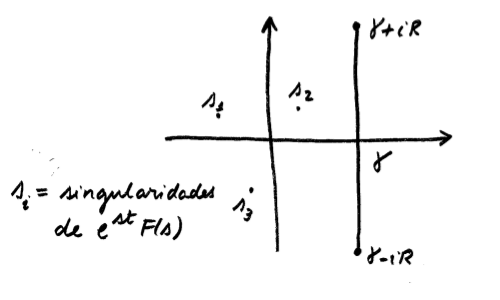
\includegraphics{figuras/14-0}
\end{figure}

Vamos calcular $I_R(t)$:
\begin{dmath*}
  I_R(t) = \frac{1}{2 \pi i} \int_{\gamma - i R}^{\gamma + i R} \exp(s t) F(s)
  \vi{s}
  = \frac{1}{2 \pi i} \int_{\gamma - i R}^{\gamma + i R} \exp(s t)
  \int_0^{\infty} \exp(-s z) f(z) \vi{z} \vi{s}
  = \frac{1}{2 \pi i} \int_0^{\infty} f(z) \int_{\gamma - i R}^{\gamma + i R}
  \exp(s (t - z)) \vi{s} \vi{z}
  = \frac{1}{2 \pi i} \int_0^{\infty} f(z) \left. \frac{\exp(s (t - z))}{t - z}
  \right|_{\gamma - i R}^{\gamma + i R} \vi{z}
  = \frac{1}{2 \pi i} \int_0^{\infty} f(z) \exp(\gamma (t - z))
  \frac{\exp(i R (t - z)) - \exp(-i R (t - z))}{t - z} \vi{z}
  = \frac{1}{\pi} \int_0^{\infty} f(z) \exp(\gamma (t - z))
  \frac{\sin(R (t - z))}{t - z} \vi{z}
  = \frac{1}{\pi} \int_{-t}^{\infty} f(t + u) \exp{-\gamma u}
  \frac{\sin(R u)}{u} \vi{u}
  = \frac{1}{\pi} \int_{-t}^0 f(t + u) \exp(-\gamma u) \frac{\sin(R u)}{u}
  \vi{u} + \frac{1}{\pi} \int_0^{\infty} f(t + u) \exp(-\gamma u)
  \frac{\sin(R u)}{u} \vi{u}
\end{dmath*}
% TODO Informar número da página.
Mas do lema das páginas ?? e ?? sabemos que
\begin{dmath*}
  \lim_{k \to \infty} \int_0^b F(u) \frac{\sin(R u)}{u} F(u) = \lim_{k \to
  \infty} \int_0^{\infty} F(u) \frac{\sin(R u)}{u} \vi{u}
  = \frac{\pi}{2} F(0^+).
\end{dmath*}
Com isso, para $R \to \infty$, temos
\begin{dgroup*}
  \begin{dmath*}
    \lim_{R \to \infty} \frac{1}{pi} \int_0^{\infty} f(t + u) \exp(-\gamma u)
    \frac{\sin(R u)}{u} \vi{u} = \frac{1}{\pi} \frac{\pi}{2} f(t + 0)
    = \frac{1}{2} f(t^+),
  \end{dmath*}
  \begin{dmath*}
    \lim_{R \to \infty} \frac{1}{\pi} \int_{-t}^0 f(t + u) \exp(-\gamma u)
    \frac{\sin(R u)}{u} \vi{u} = \begin{cases}
      0, & t = 0, \\
      (1 / 2) f(t^-), & t > 0, \\
      (-1 / 2) f(t^+), & t < 0,
    \end{cases}
  \end{dmath*}
\end{dgroup*}
de modo que
\begin{dmath*}
  \lim_{R \to \infty} I_R(t) = \begin{cases}
    (1 / 2) f(0), & t = 0, \\
    (1 / 2) [f(t^+) + f(t^0)], & t > 0, \\
    0, & t < 0.
  \end{cases}
\end{dmath*}
De fato:
\begin{dmath*}
  f(t) H(t) = \frac{1}{2 \pi i} \int_{\gamma - i \infty}^{\gamma + i \infty}
  \exp(s t) F(s) \vi{s}
\end{dmath*}
que é chamada de integral de Bromwich ou integral de Mellin ou ainda integral de
Fourier-Mellin.

\begin{exem}
  Considere
  \begin{dmath*}
    F(s) = \frac{k}{s^2 - k^2}
    = \frac{k}{(s - k) (s + k)}.
  \end{dmath*}
  Então
  \begin{dmath*}
    f(t) = \frac{1}{2 \pi i} \int_{\gamma - i \infty}^{\gamma + i \infty} \exp(s
    t) \frac{k}{s^2 - k^2} \vi{s}
    = \left[ \Res_{s = k} + \Res_{s = -k} \right] \left( \frac{\exp(s t) k}{s^2
    - k^2} \right)
    = \frac{\exp(k t) k}{2 k} + \frac{\exp(-k t) k}{(-2 k)}
    = \frac{\exp(k t) - \exp(-k t)}{2}
    = \sinh(k t).
  \end{dmath*}
  \begin{figure}[htb]
    \centering
    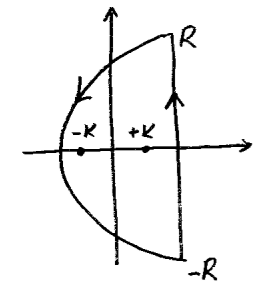
\includegraphics{figuras/14-1}
  \end{figure}
\end{exem}

\begin{exem}
  Considere $F(s) = 1 / \sqrt{s}$. Como $s = 0$ é um ponto de ramificação,
  \begin{figure}[htb]
    \centering
    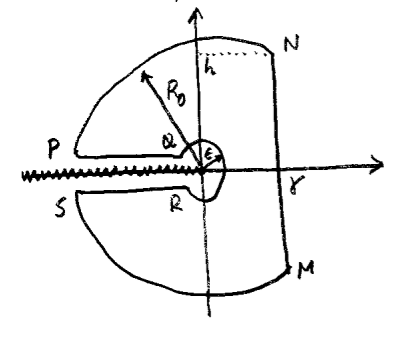
\includegraphics{figuras/14-2}
  \end{figure}
  temos
  \begin{dmath*}
    \int_M^N + \int_N^P + \int_P^Q + \int_Q^R + \int_R^S + \int_S^M = 0
  \end{dmath*}
  % TODO Terminar de digitar o exemplo. M2S12-14.pdf página 5.
\end{exem}

\begin{exem}
  Considere $F(s) = A(s) / B(s)$, com
  \begin{dmath*}
    B(s) = (s - s_1) \ldots (s - s_n) \condition{$s_1 \neq \ldots s_n$.}
  \end{dmath*}
  \begin{figure}[htb]
    \centering
    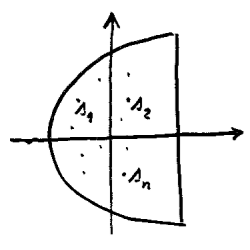
\includegraphics{figuras/14-3}
  \end{figure}
  Então,
  \begin{dmath*}
    f(t) = \frac{1}{2 \pi i} \int_{\gamma - i \infty}^{\gamma + i \infty}
    \frac{H(s) \exp(s t)}{(s - s_1) \ldots (s - s_n)} \vi{s}
    = \sum_{i = 1}^n \Res_{s = s_i} \left[ \frac{A(s) \exp(s t)}{(s - s_1)
    \ldots (s - s_n)} \right]
    = \sum_{i = 1}^n \lim_{s \to s_1} \left[ \frac{(s - s_i) A(s) \exp(s t)}{(s
    - s_1) \ldots (s - s_n)} \right]
    = \sum_{i = 1}^n \left[ \frac{A(s_i) \exp(s_i t)}{(s_i - s_1) \ldots (s_i -
    s_{i - 1}) (s_i - s_{i + 1} \ldots (s_i - s_n)} \right]
  \end{dmath*}
  Mas
  \begin{dmath*}
    B'(s) = (s - s_2) (s - s_3) \ldots (s - s_n) + (s - s_1) (s - s_3) \ldots (s
    - s_n) + \ldots + (s - s_1) (s - s_2) \ldots (s - s_{n - 1}),
  \end{dmath*}
  portanto,
  \begin{dmath*}
    B'(s_i) = (s_i - s_1) (s_i - s_2) \ldots (s_i - s_{i - 1})) (s_i - s_{i +
    1}) \ldots (s_i - s_n).
  \end{dmath*}
  Logo,
  \begin{dmath*}
    f(t) = \sum_{i = 1}^n \frac{A(s_i) \exp(s_i t)}{B'(s_i)}
  \end{dmath*}
\end{exem}

\begin{exem}
  Considere $F(s) = A(s) / (s - a)^n$.
  \begin{figure}[htb]
    \centering
    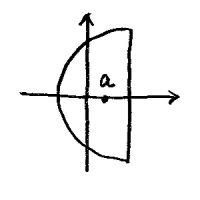
\includegraphics{figuras/14-4}
  \end{figure}
  Então,
  \begin{dmath*}
    f(t) = \frac{1}{2 \pi i} \int_{\gamma - i \infty}^{\gamma + i \infty}
    \frac{A(s) \exp(s t)}{(s - a)^n} \vi{s}
    = \Res_{s = 1} \left[ \frac{A(s) \exp(s t)}{(s - a)^n} \right]
    = \lim_{s \to a} \frac{1}{(n - 1)!} \fder{^{n - 1}}{s^{n - 1}} \left[ A(s)
    \exp(s t) \right]
    = \lim_{s \to a} \frac{1}{(n - 1)!} \sum_{k = 0}^{n - 1} \binom{n - 1}{k}
    A^{(k)}(s) t^{n - 1 - k} \exp(s t)
    = \sum_{k = 0}^{n - 1} \frac{1}{(n - 1 - k)! k!} A^{(k)}(a) t^{n - 1 - k}
    \exp(a t).
  \end{dmath*}

  Para $F(s) = A(s) / [(s - a_1)^{n_1} \ldots (s - a_i)^{n_i}]$ usamos a
  decomposição em frações parciais e aí a expressão acima para cada termo.
\end{exem}

\section{Algumas aplicações}
\begin{exem}[EDO de segunda ordem]
  Considere o sistema
  \begin{dmath*}
    \begin{cases}
      x'' + 2 \lambda x' + w_0^2 x = f(x), & w_o > \lambda, \\
      x(0) = x_0, \\
      x'(0) = v_0.
    \end{cases}
  \end{dmath*}
  Então,
  \begin{dgroup*}
    \begin{dmath*}
      \mathcal{L}[x'] = s \mathcal{L}[x] - x(0)
      = s X(s) - x_0,
    \end{dmath*}
    \begin{dmath*}
      \mathcal{L}[x''] = s^2 \mathcal{L}[x] - s x(0) - x'(0)
      = s^2 X(s) - s x_0 - v_0.
    \end{dmath*}
  \end{dgroup*}
  Portanto,
  \begin{dgroup*}
    \begin{dmath*}
      F(s) = s^2 X(s) - s x_0 - v_0 + 2 \lambda s X(s) - 2 \lambda x_0 + w_0^2
      X(s),
    \end{dmath*}
    \begin{dmath*}
      F(s) = \left( s^2 + 2 \lambda s + w_0^2 \right) X(s) - \left( 2 \lambda +
      s \right) x_0 - v_0,
    \end{dmath*}
    \begin{dmath*}
      X(s) = \frac{(2 \lambda + s) x_0 + v_0}{s^2 + 2 \lambda s + w_0^2} +
      \frac{F(s)}{s^2 + 2 \lambda s + w_0^2}.
    \end{dmath*}
    Mas:
    \begin{dmath*}
      s^2 + 2 \lambda s + w_0^2 = 0
    \end{dmath*}
    cuja solução é
    \begin{dmath*}
      s = - \lambda \pm i \sqrt{w_0^2 - \lambda^2} \condition{$w_0 > \lambda$.}
    \end{dmath*}
    % TODO Completar exemplo. M2S12-14.pdf pyágina 10.
  \end{dgroup*}
\end{exem}

\begin{exem}[EDP: Equação de Difusão]
  Considere o sistema
  \begin{dmath*}
    \begin{cases}
      \pder{u}{t} = \frac{1}{k^2} \pder{^2 u}{x^2}, & t \geq 0, x \geq 0, \\
      u(x, 0) = T_0, \\
      u(0, t) = T_1, \\
      \lim_{x \to \infty} u(x, t) < +\infty.
    \end{cases}
    % TODO Completar exemplo. M2S12-14.pdf pyágina 13.
  \end{dmath*}
\end{exem}

\begin{exem}
  A transformada de Laplace é particularmente útil para estudarmos expansões
  assintóticas. Dizemos que $\sum_{k = 0}^{\infty} a_k / z^k$ é uma expansão
  assintótica de $f(x)$ se
  \begin{dmath*}
    \lim_{\lvert z \rvert \to \infty} z^n \left[ f(z) - \sum_{k = 0}^n \frac{a_k}{z^k}
    \right] = 0 \condition{$n = 0, 1, 2, \ldots$,}
  \end{dmath*}
  e escrevemos
  \begin{dmath*}
    f(z) \sim \sum_{k = 0}^{\infty} \frac{a_k}{z^k}.
  \end{dmath*}

  Vamos supor que $f(t)$ tem a seguinte expansão em série de Taylor:
  \begin{dmath*}
    f(t) = \sum_{n = 0}^{\infty} a_n t^{\lambda_n - 1},
  \end{dmath*}
  onde $0 < \lambda_0 < \lambda_1 < \ldots$, e que seja de ordem exponencial
  para $t > a$,
  \begin{dmath*}
    \lvert f(t) \rvert < c \exp(b t).
  \end{dmath*}
  Seja agora
  \begin{dmath*}
    f_n(t) = f(t) - \sum_{k = 0}^n a_k t^{\lambda_k - 1}.
  \end{dmath*}
  Em função desses comportamentos para $t \to 0$ e $t > a$, existem constantes
  tais que
  \begin{dmath*}
    \lvert f_n(t) \rvert \leq c_n \exp(b t) t^{\lambda_{n + 1} - 1}.
  \end{dmath*}
  Por outro lado,
  \begin{dmath*}
    \mathcal{L}[f_n(t)] = \mathcal{L}[f(t)] - \sum_{k = 0}^n a_k L[t^{\lambda_k
    - 1}]
    = \mathcal{L}[f(t)] - \sum_{k = 0}^n a_k
    \frac{\Gamma(\lambda_k)}{s^{\lambda_k}}
  \end{dmath*}
  de modo que, se
  \begin{dmath*}
    \lim_{\lvert s \rvert \to \infty} \lvert s \rvert^{\lambda_n} \lvert
    \mathcal{L}[f_n(t)] \rvert = 0
  \end{dmath*}
  então temos
  \begin{dmath*}
    F(s) = \mathcal{F}[f(t)]
    \sim \sum_{k = 0}^{\infty} a_k \frac{\Gamma(\lambda_k)}{s^{\lambda_k}}.
  \end{dmath*}
  De fato:
  \begin{dmath*}
    \lvert\mathcal{L}[f_n(t)]\rvert \leq \int_0^{\infty} \lvert\exp(-s
    t)\rvert \lvert f_n(t) \rvert \vi{t}
    \leq \int_0^{\infty} \exp(-\Re(s) t) c_n \exp(b t) t^{\lambda_{n + 1} - 1}
    \vi{t}
    \leq c_n \int_0^{\infty} \exp(-\lvert s \rvert \cos(\varphi t) \exp(b t) t^{\lambda_{n
    + 1} - 1} \vi{t}
    = c_n \frac{\Gamma(\lambda_{n + 1}}{(\lvert s \rvert \cos(\varphi) - b)^{\lambda_{n +
    1}}},
  \end{dmath*}
  onde devemos ter $\lvert s \rvert \cos(\varphi) - b > 0$, o que
  necessariamente implica que $\cos(\varphi) > 0$, ou seja, $\arg(s) < \pi / 2$.

  Com isso,
  \begin{dmath*}
    \lim_{\lvert s \rvert \to \infty} \lvert s \rvert^{\lambda_{n}} \lvert
    \mathcal{L}[f_n(t)] \rvert \leq \lim_{\lvert s \rvert \to \infty}
    \frac{\lvert s \rvert^{\lambda_n} c_n \Gamma(\lambda_{n + 1})}{(\lvert s
    \rvert \cos(\varphi) - b)^{\lambda_{n + 1}}}
    = 0.
  \end{dmath*}
  Portanto, provamos o chamado Lema de Watson, ou seja, se $f(t) = \sum_{n =
  0}^{\infty} a_n t^{\lambda_{n - 1}}$ e é de ordem exponencial, então a sua
  transformada de Laplace $F(s)$ tem, para $\arg(s) < \pi / 2$, a segute
  expressão assintótica:
  \begin{dmath*}
    F(s) = \mathcal{L}[f(t)] \sim \sum_{k = 0}^{\infty} a_k
    \frac{\Gamma(\lambda_k)}{s^{\lambda_k}}.
  \end{dmath*}
  Por exemplo, para $f(t) = \ln(1 + \sqrt(t))$, temos
  \begin{dmath*}
    \ln(1 + \sqrt(t)) = \sum_{n = 1}^{\infty} \frac{(-1)^{n + 1} (\sqrt{t})^n}{n}
  \end{dmath*}
  e daí
  \begin{dmath*}
    \mathcal{L}[\ln(1 + \sqrt{t})] \sim \sum_{n = 1}^{\infty}
    \frac{(-1)^{n + 1}}{n} \frac{\Gamma(n / 2 + 1)}{s^{n / 2 + 1}}.
  \end{dmath*}
\end{exem}
